% Main Thesis File: This is the main file and it connects all the different parts of the thesis and compiles it into a single outcome file.

\documentclass[onecolumn, 12 pt, doublespace, fullpage, a4paper]{report}
\renewcommand{\baselinestretch}{1.75} % baseline stretch

% Packages
\usepackage{amssymb}
\usepackage{amsthm}
\usepackage[cmex10]{amsmath}
\usepackage{adjustbox} 
\usepackage{arabtex} 
\usepackage{academicons}
\usepackage{breakcites} 
\usepackage{color}
\usepackage{epsfig}
\usepackage{epstopdf}
\usepackage{etoolbox}
\usepackage{enumitem}
\usepackage{float}
\usepackage{fancyhdr}
\usepackage{graphicx}
%for \includegraphics[]{picturename.filetype} command
\usepackage{graphics}
%\usepackage[breaklinks]{hyperref} % if you want to highlight the links
%\usepackage[hidelinks]{hyperref}
\usepackage{latexsym,amsfonts}
\usepackage{longtable}
\usepackage{listings}
\usepackage{lscape} 
\usepackage{lipsum}
\usepackage{multirow}             
\usepackage{pdfpages}
\usepackage[figuresright]{rotating} 
\usepackage{sectsty}
\usepackage{setspace}
\usepackage{subfigure}
\usepackage{textcomp}
\usepackage{utf8} 
\usepackage[hyphens]{url} 
\usepackage{wrapfig} 
\usepackage{wasysym} 
\usepackage{xcolor}
\usepackage[table,xcdraw]{xcolor}
%listset command to insert code [from Stack Overflow]%
\definecolor{dkgreen}{rgb}{0,0.6,0}
\definecolor{gray}{rgb}{0.5,0.5,0.5}
\definecolor{mauve}{rgb}{0.58,0,0.82}

\lstset{frame=tb,
  language=Mathematica,
  aboveskip=3mm,
  belowskip=3mm,
  showstringspaces=false,
  columns=flexible,
  basicstyle={\small\ttfamily},
  numbers=none,
  numberstyle=\tiny\color{gray},
  keywordstyle=\color{blue},
  commentstyle=\color{dkgreen},
  stringstyle=\color{mauve},
  breaklines=true,
  breakatwhitespace=true,
  tabsize=3
}

% you can define your most used synonyms/acronyms
\def\KAUST {King Abdullah University of Science and Technology}
\def\dg{$^\circ$}		 % for degree celcius
\def\2{$^2$}			 % for raised to power 2
\def\3{$^3$}			 % for raised to power 3
\def\-2{$^{-2}$}		 % for raised to power -2
\def\-3{$^{-3}$}		 % for raised to power -2
\def\-1{$^{-1}$}		 % for raised to power -1
\def\h{W.m$^{-2}$K$^{-1}$}
\def\hh{kJ.kg$^{-1}$}
\def\hfg{kJ.kg$^{-1}$}
\def\ss{kJ.kg$^{-1}$K$^{-1}$}
\def\Q{W.m$^{-2}$}
\def\mone {$^{-1}$}
\def\mtwo {$^{-2}$}
\def\um{$\mu m$}
\def\kwhm{kWh.m$ ^{-3} $}
\def\LMH{kg.m$^{-2}$h$^{-1}$}


% Changing chapters' headings and subheadings to size 14
\chapterfont{\fontsize{14}{15}\selectfont}   % font size and baseline stretch
\sectionfont{\fontsize{14}{15}\selectfont}
\subsectionfont{\fontsize{14}{15}\selectfont}
\subsubsectionfont{\fontsize{14}{15}\selectfont}

       
\pagestyle{fancy} % adds a line at the top of every page, except title-page
\fancyhead{} \fancyfoot{} % for header and footer
\fancyfoot[CO,CE]{\thepage}    % center odd and even page number

%centering the page numbers with text body
\fancyheadoffset[L]{0.01mm}
\renewcommand{\headrulewidth}{0pt}


%The following code changes the empty vertical space above a new chapter title. It sets it from 50pt to 20pt
\makeatletter
\patchcmd{\@makechapterhead}{50\p@}{20pt}{}{}
\patchcmd{\@makeschapterhead}{50\p@}{20pt}{}{}
\makeatother
%end of modification



% The following code redefines the plain pagestyle with the objective of moving the page number from the bottom to the top of the page. This only affects new chapter pages.
\fancypagestyle{plain}{
\fancyhf{} %clear all header and footer fields
\fancyhead[C]{\thepage} %puts number on top center of the page
\renewcommand{\headrulewidth}{0pt}
\renewcommand{\footrulewidth}{0pt}}
%ending of plain pagestyle modification.




% ### Nomenclature, List of Abbreviations and List of Symbols 
   \usepackage{ifthen,xkeyval,xfor,amsgen}
   \usepackage[acronym,toc, nogroupskip]{glossaries}
   \newglossary[slg]{symbols}{syi}{sbl}{List of Symbols}
 
   \makeglossaries
   
   
% #### Symbols ####
\newglossaryentry{symb:Pi}{
name=$\pi$, type=symbols,
description=A mathematical constant whose value is the ratio of any circle's circumference to its diameter,
sort=symbolpi
}

\newglossaryentry{symb:Phi}{
name=$\varphi$, type=symbols,
description=An angle,
sort=symbolphi
}

\newglossaryentry{symb:Lambda}{
name=$\lambda$, type=symbols,
description=Lambda indicates usually an eigenvalue in linear algebra,
sort=symbollambda
}

% #### Abbreviations ####
\newacronym{toc}{ToC}{Table of Contents}
\newacronym{los}{LoS}{List of Symbols}
\newacronym{loa}{LoA}{List of Abbreviations}
\newacronym{phd}{PhD}{Doctoral}
\newacronym{MS}{MS}{Masters}
\newacronym{M$}{MS}{Microsoft}
\newacronym{CD}{CD}{Compact Disc}
\newacronym{kaust}{KAUST}{King Abdullah University of Science and Technology}

%An acronym with a glossary entry
\newacronym{AD}{AD}{Active Directory\protect\glsadd{glos:AD}}



% #### Nomenclature terms ####
\newglossaryentry{glos:AD}{
name=Active Directory,
description={Active Directory is the directory service for Windows based networks, that allows central organization and administration of any network resource. It allows a single-sign-on concept independent from network topologies or network protocols. As a prerequisite you need a Windows Server acting as Domain Controller. This computer stores all necessary data, e.g.~usernames and corresponding passwords}
}

\newglossaryentry{glos:RespF}{name=response file, description={A file 
that allows unattended software installation}}


   % Run the following three lines in the command line to get the lists
%makeindex -s Thesis.ist -t Thesis.alg -o Thesis.acr Thesis.acn
%makeindex -s Thesis.ist -t Thesis.slg -o Thesis.syi Thesis.sbl
%makeindex -s Thesis.ist -t Thesis.glg -o Thesis.gls Thesis.glo

% ### End of addition




% Modified commands
\newcommand{\Tab}{\hspace{2ex}}
\usepackage[lmargin=40mm, rmargin=25mm, vmargin=25mm, headsep=2.5mm]{geometry}
\newcommand{\mathsym}[1]{{}}
\newcommand{\unicode}[1]{{}}
\renewcommand{\thechapter}{\arabic{chapter}}
\renewcommand\bibname{\centering BIBLIOGRAPHY}
%\newcommand{\orcid}[1]{\href{https://orcid.org/#1}{\textcolor[HTML]{A6CE39}{\aiOrcid}}}
\newcommand{\orcid}{
\includegraphics[width=8pt]{ORCID}} % ORCID ID


\begin{document}

% $$$$$$$$$$$$$$$$$  Start of Thesis Front matter   $$$$$$$$$$$$$$

%\vspace{10mm}  % vertical space
\thispagestyle{empty}
\addvspace{5mm}  % vertical space until length

%$$$$$$$$$$$$$$$$$$$$$$$$$$$$$$$$$$$$$$$$$$$$$$$$$$$$$$$$$$$$$$$$$$$$$$$$$$$$$$$$$

% make the title page
\begin{center}
\begin{doublespace}
{\textbf{{\large Applications of Cubic Spline Interpolation On Functions in Normed Spaces}}}%\vfill % Write your thesis title
\end{doublespace}

\vspace{10mm}
{A Thesis by}\\
{Cory Suzuki}\\
{May 8, 2023}%\vfill

\vspace{30mm}

{ In Partial Fulfillment of the Requirements}\\[12pt]
{ For the Certificate Bestowed By}\\[12pt]
{University Honors Program} \vfill
{California State University, Long Beach }\\
{California, United States of America}\\
{This thesis has been approved by}\\
{Dr. Kathryn McCormick}
\vfill

\end{center}
% end of title page
%$$$$$$$$$$$$$$$$$$$$$$$$$$$$$$$$$$$$$$$$$$$$$$$$$$$$$$$$$$$$$$$$$$$$$$$$$$$$$$$$$
\newpage

%$$$$$$$$$$$$$$$$$$$$$$$$$$$$$$$$$$$$$$$$$$$$$$$$$$$$$$$$$$$$$$$$$$$$$$$$$$$$$$$$$

%
\begin{center}
\begin{doublespace}
{\textbf{{\large I, THE UNDERSIGNED MEMBER OF THIS COMMITTEE, HAVE APPROVED THIS THESIS}}}%\vfill % Write your thesis title
\end{doublespace}

\vspace{10mm}
{Applications of Cubic Spline Interpolation On Functions in Normed Spaces}\\
{By Cory Suzuki}\\
%\vfill

\vspace{30mm}
 \vfill
 \hrulefill \newline
{Kathryn McCormick, Ph.D. (Thesis Advisor)}\\
{Dept. of Mathematics and Statistics}\\
{California State University, Long Beach}\\
{Spring 2023}\\
\vfill

\end{center}
% end of title page
%$$$$$$$$$$$$$$$$$$$$$$$$$$$$$$$$$$$$$$$$$$$$$$$$$$$$$$$$$$$$$$$$$$$$$$$$$$$$$$$$$
\newpage

\chaptertitlefont{\fontsize{14}{15}\selectfont\centering}  



% Abstract File
% Do not remove centering environment below
\begin{center}

\end{center}

\begin{center}
{{\bf\fontsize{14pt}{14.5pt}\selectfont \uppercase{ABSTRACT}}}
\end{center}

\doublespacing
\addcontentsline{toc}{chapter}{Abstract}



\begin{center}
	\begin{doublespace}
%{\fontsize{14pt}{14.5pt}\selectfont {Applications of Cubic Spline Interpolation On Functions in Normed Spaces}}\\
		%{\fontsize{14pt}{14.5pt}\selectfont {Cory Suzuki}}\\
%		{\fontsize{12pt}{12.5pt}\selectfont {Ph.D. Year}}\\
	\end{doublespace}
\end{center}


In this paper, we conduct a detailed error analysis of two cubic spline interpolation methods described in Kreyszig and Mhaskar-Pai in the $L^2$ and $L^{\infty}$ norms. We begin by introducing the basic theory of cubic spline interpolation and dissecting each of the interpolation conditions from both methods. The data was collected by constructing splines of various elementary functions and calculating the relative $L^2$ and $L^{\infty}$ error between each function and its spline. The numerical data has shown that the functions $x^4$, $\cos(x)$, and $\ln(x+1)$ using both methods of interpolation approximate their functions with minimal relative error. We show that polynomial-trigonometric functions are the worst in the $L^2$ and $L^{\infty}$ norms. We conjecture that higher-order powers of polynomial-trigonometric functions such as $x^n\sin(x)$ will always perform worse than the polynomial function $x^{n}$ in the $L^2$ and $L^{\infty}$ norms. In addition, we compared the actual Mhaskar-Pai error to the error bounds given in \cite[pg.~269]{key5}. We observe how sharp the bound was for various elementary functions.
  % include your abstract file



% Acknowledgments File


\begin{center}

\end{center}
\begin{center}

{\bf\fontsize{14pt}{14.5pt}\selectfont \uppercase{Acknowledgements}}\\\vspace{1cm}
\end{center}

\addcontentsline{toc}{chapter}{Acknowledgements} % (Optional)





I would like to personally express my gratitude to all participating parties who have made this project possible. Firstly, to Dr. McCormick, my thesis advisor and introductory proofs class professor. My success in upper-division classes like real analysis and abstract algebra can be traced back to your lectures. Thank you for dedicating your time and effort to guiding me through the process of writing my very first thesis, something that I never saw myself doing. I am grateful for your patience and feedback in reviewing all the pages of each document and providing advice in writing the Mathematica code to collect the necessary data needed for this thesis.

Secondly, thank you to my parents and grandmother for being an inspiration to go beyond the limits of my own potential. Without their words of encouragement and belief in my abilities, I would not have been able to finish or even continue the thesis during the many times of struggling with getting things right. Thank you for giving me reassurance during all the times I got overwhelmed with all the calculations and lines of code.

Thirdly, I would like to thank Dr. Murray for not only being my Honors Calculus III professor but for also being a huge inspiration and mentor in the field of mathematics. It is your enthusiastic energy and amazing lectures that have fueled my thirst for knowledge from basic mathematics all the way to introductory ring theory. Thank you for your time talking to me even outside of office hours, and I hope to learn so much more about the curiosities that mathematics has to offer.

  % include your Acknowledgement file


\begin{onehalfspacing}%To make the table of contents, figures, and tables single spaced, as required by the formatting guidelines, pg. 24.

%\renewcommand{\contentsname}{\textbf{{\large TABLE OF CONTENTS}}}
\tableofcontents
% Maybe we don't need this blank page.
%\cleardoublepage

\printglossary[type=\acronymtype,style=long3col, title=\centerline{LIST OF ABBREVIATIONS}, toctitle=List of Abbreviations, nonumberlist=true] 

\printglossary[type=symbols,style=long3col, title=\centerline{LIST OF SYMBOLS}, toctitle=List of Symbols, nonumberlist=true]


\end{onehalfspacing}
% \printglossary[style=altlist,title=Nomenclature, toctitle=Nomenclature, nonumberlist=true] 

% $$$$$$$$$$$$$$$$$  Thesis front matter ends   $$$$$$$$$$$$$$



% $$$$$$$$$$$$$$$$$  include your separate chapters   $$$$$$$$$$$$$$
% Remove the centering of chapter name.
\chaptertitlefont{\fontsize{14}{15}\selectfont}  % <------ Add this line


% Chapter 2 File

\chapter{Introduction}
\label{chapter1}
\thispagestyle{empty}

 Approximation theory is a field of mathematics that studies special algorithms that aid mathematicians and scientists in making approximations of objects like functions and data. Functions in particular are quite interesting as they represent real-life phenomena as abstractions, which in turn are then used to predict other natural phenomena. Without approximation theory, we would not have many important inventions such as spaceships, airplanes, and computers which we often take advantage of.
\\\\
An \emph{algorithm} is a well-defined list of steps that are used to produce an effective solution to a specific problem instance. Algorithms are malleable and can be modified to solve other similar problem instances. For example, consider the Newton-Raphson and the Secant algorithms, which originate from the field of numerical analysis. These algorithms are used to approximate the roots of functions on specific domains with appropriately defined tolerance values. They both achieve this goal, so we say that these algorithms belong to a \emph{class} of problem instances, in this case, root approximation. However, it is important to note that these algorithms do not solve the same problem instance. The Newton-Raphson algorithm requires that the derivative of a function be known, unlike the Secant algorithm which utilizes the secant variation of the derivative definition in its process \cite{key3}. Knowing what an algorithm is, we now introduce the motivation for researching cubic spline interpolation. We will be interested in studying two different algorithms for constructing cubic splines and analyzing the approximation of elementary functions in the $L^2$ and $L^{\infty}$ norms.


\section{Motivation for Research: Why Do We Study Cubic Splines?}
The fields of approximation theory and functional analysis are fundamentally crucial in understanding how accurate the approximations of functions are. With these tools in our arsenal, we have the ability to provide accurate estimates of arbitrary functions and compute the errors in such calculations. The type of approximation we primarily study is \emph{cubic spline interpolation}. This method of approximation has been proven useful in recent developments such as filling in missing portions of weather data using the statistical method of time series \cite{key1}. Another significant motivation for studying splines is that basis spline interpolation is utilized for image processing and digital filtering \cite{key2}.
\\\\
We want to study how we can use certain algorithms from approximation theory in order to make accurate approximations of both known and unknown functions. We denote \emph{known functions} to be functions that you may recall from high school such as polynomials and logarithms, while \emph{unknown functions} are functions that may be a combination of elementary known functions, or may even be defined piece-wise based on data. This leads us to the heart of the research on the effectiveness of cubic spline interpolation. A cubic spline can be utilized to our advantage by producing approximations of functions and observing how well they estimate said functions. For instance, we are interested in finding the approximation error and comparing that to the upper bounds established in the literature. Another factor we will consider is how changing the number of data points in a partition effects the approximation. These questions will guide our research on how cubic spline interpolation can be optimized under hypothetical constraints. 

% Chapter 3 File

\chapter{Preliminaries and Background}
\label{chapter2}
\thispagestyle{empty}

\section{Background}
Cubic spline interpolation is a type of numerical mathematical method in which a function's domain is divided into pieces by a partition and a polynomial is fitted onto each piece. These polynomials are chosen to have a maximum degree of 3. Interpolation refers to the idea that the cubic spline function (also known as the \emph{interpolant}) passes through each of the points of the graph of the function being approximated for the $x$-values in the partition. The advantage of this type of approximation is that these types of problems require a limited amount of information. For example, for the most basic cubic spline on a partition of size $n$ we only need $n+1$ data points rather than all of the values of the function. In addition, it is necessary that boundary conditions are placed on the function's derivative if you would like to guarantee the smoothness of the resulting spline function. This is evident by the definition of a cubic spline that Erwin Kreyszig provides in \emph{Introductory Functional Analysis with Applications} in which the values of each derivative must agree on the chosen partition \cite[pg.~358]{key4}. An interesting property of spline approximations is that while they are defined piece-wise, their approximation together within the given interval $[a,b]$ can ultimately fail to be accurate if the function being approximated has too many points of fluctuation or oscillation \cite[pg.~28]{key8}. In extreme cases, it may be more appropriate to use a non-cubic spline function, such as a rational function, which may be more accurate when approximating trigonometric functions. This problem may arise even within the chosen interval of interpolation, as specified in M. J. D. Powell's text on approximation theory \cite[pg.~28]{key8}.
\\\\
There are three popular methods of determining how accurate a cubic spline approximation is, namely with the $L^1$, $L^2$, and the $L^\infty$ norms. An important theorem in the literature illustrates that if the function $f$ is infinitely differentiable, or in simpler terms a \emph{smooth function}, then there is a spline interpolant that is a second-order approximation of $f$ with respect to the $L^2$ and $L^\infty$ norms respectively \cite[pg.~19]{key9}. This theorem is especially helpful since it establishes useful norms in constructing cubic splines and conducting the error analysis of cubic spline functions. Gunther N\"{u}rnberger in his work \emph{Approximation by Spline Functions} says that the best $L^{2}$ spline approximations are always unique and can be solved via a system of linear equations in finite-dimensional spaces \cite[pg.~76]{key6}.
\section{Introduction to Metric Spaces $\&$ Normed Spaces}
\emph{Definition 1.1.} Let S be a nonempty set and let $d$ be a real-valued function $d:S \times S \rightarrow \mathbb{R} $ such that the following axioms apply:\newline
$(i)\ d(x,y) \geq 0 \ \forall x,y \in \mathbb{R}$\\
$(ii)\ d(x,y)=0  \iff \ x=y$\\
$(iii)\ d(x,y)=d(y,x)$\\
$(iv)\ d(x,z)=d(x,y)+d(y,z)$\newline\\
Then we say that $(S,d)$ is a \emph{metric space} \cite{key7}. It is interesting to note that the real-valued function $d$ is called a metric since it measures the non-negative distance between two points in $S$. We now move on to the definition of a complete metric space, a norm \cite[pg. 438]{key3}, and a normed space before proceeding with the definition of a Banach space.
\\\\
\emph{Definition 1.2.} A \emph{norm} is a function $\|\cdot\|:\mathbb{R}^{n} \rightarrow \mathbb{R}$ that obeys the following properties:\newline
$(i)\ \|\textbf{x}\| \geq 0 \ \forall \textbf{x} \in \mathbb{R}^{n}$\\
$(ii)\ \|\textbf{x}\|=0  \iff \ \textbf{x}=0$\\
$(iii)\ \|\alpha\textbf{x}\| = \|\alpha\|\|\textbf{x}\| \ \forall \alpha \in \mathbb{R} \ \text{and} \ \textbf{x} \in \mathbb{R}^{n}$\\
$(iv)\ \|\textbf{x}+\textbf{y}\| \leq \|\textbf{x}\|+\|\textbf{y}\| \ \forall \textbf{x}, \textbf{y} \in \mathbb{R}^{n}$\newline
\\\\
\emph{Example.} A normed space $(S,\|\cdot\|)$ is a metric space with the metric $d(x,y)=\|x-y\|$. \newline
Furthermore, a metric space $(S,d)$ is \emph{complete} if every Cauchy sequence converges in the space. A \emph{Banach space} is a complete normed vector space.
\\\\
 Here we will mainly focus on Banach spaces that contain the continuous functions $C[a,b]$. This leads us to our first theorem, which tells us an important property of the space $C[a,b]$.
\\\\
\emph{Theorem 1.1.} Let $[a,b] \subset \mathbb{R}.$ The function space $C[a,b]$ is complete under the norm $\displaystyle{\|f-g\|_{\infty}=\max_{t \in [a,b]} |f(t)-g(t)|}$.
\\\\
\emph{Proof.} \ Let \ $\epsilon > 0$. Suppose $(x_{m})$ is any arbitrary Cauchy sequence in $C[a,b]$. Now by definition, there exists an $N$ in $\mathbb{N}$ such that for $m,n > N$,\\
$\displaystyle{d(x_{m},x_{n})= \max_{t \in [a,b]} |x_{m}(t)-x_{n}(t)| < \epsilon}$. So for any fixed $t_o \in [a,b]$, we have
$|x_{m}(t_o)-x_{n}(t_o)| < \epsilon \hspace{0.25cm} \text{for} \ m,n > N$.
The sequence ${x_n(t_o)}$ is hence a Cauchy sequence in $\mathbb{R}$ and so we say it converges to the number $x(t_o)$. Note that this convergence applies as $m \rightarrow \infty$. So for each $t_o$, $|x_m(t_o)-x(t_o)| < \epsilon$ for $m > N$. Now we have
$\displaystyle{\max_{t \in [a,b]} |x_{m}(t)-x(t)| < \epsilon} \hspace{0.25cm} \text{for} \ m > N$.
Consequently, we have shown that the Cauchy sequence ${x_m}$ converges to the function $x$. We would then need to show that the function $x$ is continuous, please see \cite{key4} for this part of the proof. Once we show that, we then conclude that the function space $C[a,b]$ is complete. $\blacksquare$\\\\
\section{$L^p$ Norms}
To properly analyze how well cubic spline functions perform in approximating functions in normed spaces, we must introduce the $L^2$ and $L^{\infty}$ norms which will measure the error in between the cubic splines and the functions they are approximating.\\\\
\emph{Definition 2.1.} Let $f(x)$ be a real-valued, continuous function defined on the interval $[a,b]$. Then the $L^2$ norm of $f$ is defined as \newline
\\
\[\|f\|_2 = \left(\int_{a}^{b}|f(x)|^2\mathrm{d}x\right)^{\frac{1}{2}}\]\newline
\\
We can see that the $L^2$ norm is well-defined for continuous functions since $|f(x)|^2$ is also continuous in $[a,b]$, so by \cite[pg.~155]{key7} the integral exists.\\\\
\emph{Definition 2.2.} Let $f(x)$ be a real-valued, continuous function defined on the interval $[a,b]$. Then the $L^{\infty}$ norm of $f$ is defined as \newline\\
\[\|f\|_{\infty} = \max_{t \in [a,b]} |f(x)|\]\\
Note that this norm is also well-defined on continuous functions since $f(x)$ achieves its maximum on the interval $[a,b]$ by \cite[pg.~106]{key7}. More information and proofs about these norms are provided by Kreyszig \cite[pg.~61]{key4}.

% Chapter 4 File

\chapter{Cubic Spline Interpolation and Theory}
\label{chapter3}
\thispagestyle{empty}

\section{Cubic Spline Definitions $\&$ Theorems}
We will continue by providing important definitions and theorems on cubic spline functions. First, we must establish a more rigorous definition of cubic spline interpolation.
\\\\
\emph{Definition 3.1.} Let $[a,b] \subset \mathbb{R}$. Then a \emph{partition} $P_n$ on $[a,b]$ is an ordered list of real numbers:
\\\\
\centerline{$ a=x_o < x_1 < x_2 < ... < x_{n-1} < x_{n}=b$}
\\\\
 Let $[a,b] \subset \mathbb{R}$, and let $P_n$ be a partition of $[a,b]$. A \emph{cubic spline} is a function $y \in C[a,b]$ such that $y|_{[x_{i}, x_{i+1}]}$ is a cubic polynomial.\newline
 \emph{Definition 3.2} We say that a function $g(x)$ \emph{interpolates} the data points $(x_i, y_i)$ for $i= 0,...,n$ when
\\\\
\centerline{$g(x_i)=y_i \hspace{4cm} \text{for} \ i=0,...,n$}
\\\\
\emph{Definition 3.3} We define the cubic spline space presented by Kreyszig as $S(K, P_{n})$ where $g$ is in $S(K, P_{n})$ if $g$ is a cubic spline on $P_n$ and $g \in C^2[a,b]$. \newline
\emph{Definition 3.4} We define the cubic spline space presented by Mhaskar-Pai as $S(MP, P_{n})$ where $g$ is in $S(MP, P_{n})$ if $g$ is a cubic spline on $P_{n}$ and $g \in C^1[a,b]$.
\\\\
Definition 3.2 tells us more about what cubic spline interpolation is and leads to the following theorems:
\\\\
\emph{Theorem 3.2.} \cite[pg.~358]{key3} Let $f(x)$ be a real-valued function on $[a,b]$. Define $P_{n}$ to be a partition of $[a,b]$ as referenced in Definition 1.3. Suppose $a_o, a_{n} \in \mathbb{R}$. Then there is a unique cubic spline function $g(x) \in S(K, P_{n})$ such that
\\\\
\centerline{(a) $g(x_{i})=f(x_{i})$} \newline
\centerline{(b) $g'(x_o)=a_o$} \newline
\centerline{(c) $g'(x_{n})=a_{n}$} \newline
for $i=0,1,...,n$. In particular, this holds if $f$ is differentiable and $a_{o} = f'(x_{o})$ and $a_{n} = f'(x_{n})$.
\\\\
\emph{Definition 3.5} \cite{key5} Here the Sobolev spaces $W^4_{p}[a,b]$ are subspaces of the Banach space $L^{p}[a,b]$ and include $C[a,b]$ as a subset.\\\\
\emph{Theorem 3.3} \cite[pg.~267]{key5} Let $f(x)$ be a real-valued function in $C[a,b]$. Define $P_{n}$ to be a partition of $[a,b]$ as referenced in Definition 1.3. Suppose $g(x) \in W^{4}_{2}$. Then there is a unique cubic spline function $g(x) \in S(MP, P_{n})$ such that
\\\\
\centerline{(a) $g(x_{i})=f(x_{i})$} \newline
\centerline{(b) $g'(x_{i})=f'(x_{i})$} \newline
for $i=0,1,...,n$.
\\\\
We will now introduce two error estimate theorems for cubic spline interpolants that are referenced in Mhaskar and Pai's \emph{Fundamentals of Approximation Theory} \cite[pg.~269]{key5}.
\\\\
\emph{Definition 3.6} Let $P_{n}$ be a partition.\newline Then we define $\|P_{n}\| = \sqrt{(x_{1}-x_{o})^2+(x_{2}-x_{1})^2+...+(x_{n}-x_{n-1})^2}$.\\\\
\emph{Theorem 3.4.} If $f \in W^{4}_{2}[a,b]$ and $I(f)$ is the unique cubic spline from theorem 3.2, then\\
$\|f-I(f)\|_{2} \leq (\frac{\|P_{n}\|}{\pi})^4\|f^{(4)}\|_{2}$.\\\\
\emph{Theorem 3.5.} If $f \in W^{4}_{\infty}[a,b]$, and $I(f)$ is the unique cubic spline from theorem 3.3 then\\
$\|f-I(f)\|_{\infty} \leq \frac{\|P_{n}\|^{4}}{384}\|f^{(4)}\|_{\infty}$.\\\\
This concludes the main definitions and theorems that we will be utilizing in answering our questions. To clarify how we find cubic splines, we will conclude this chapter with a practical example of using a cubic spline to approximate a function.

\section{Example of a Cubic Spline for $S(K, P_{n})$}
In this section, we will provide an example of finding a cubic spline in $S(K, P_{n})$. Let $f(x)=x^4$ be a function defined on the interval $[0,2]$ and let $P=\{0,1,2\}$ be the data points that partition the interval. It's one cubic spline with $2$ pieces. The piece $p_1$ will be defined on $[0,1]$ and the other denoted by $p_2$ on $[1,2]$. To find the $p_1$ and $p_2$ which are cubics, we will need to find $4$ coefficients for each, for a total of $8$ coefficients. Using Theorem 1.2 will result in the creation of $8$ conditions for finding the coefficients $a_{o},...,d_{1} \in \mathbb{R}$ for:\\\\
\begin{equation}
p(x) = \begin{cases}
p_1(x)= a_{o}x^3+b_{o}x^2+c_{o}x+d_{o} & \text{if } x \in [0,1]\\
p_2(x)= a_{1}x^3+b_{1}x^2+c_{1}x+d_{1} & \text{if } x \in [1,2]
\end{cases}
\end{equation}\\\\
We will need to satisfy the conditions:\\
$p_1(0)=f(0)$\newline
$p_1(1)=f(1)$\newline
$p_2(1)=f(1)$\newline
$p_2(2)=f(2)$\newline
$p_1'(0)=f'(0)$\newline
$p_2'(2)=f'(2)$\newline
$p_1'(1)=p_2'(1)$\newline
$p_1''(1)=p_2''(1)$\\\\
These conditions, when plugged into the equations for $p_1(x)$, $p_2(x)$, and $f(x)$, will result in a system of $8$ linear equations that can be solved via Gaussian elimination or through a computer program. A program in the Mathematica language is provided in Appendix A which can be used to find the coefficients. For this particular example, the cubic spline function for $f(x)$ is given by equation 3.2:\\\\
\begin{equation}
p(x) = \begin{cases}
p_1(x)=2x^3-x^2 & \text{if } x \in [0,1]\\
p_2(x)=6x^3-13x^2+12x-4 & \text{if } x \in [1,2]
\end{cases}
\end{equation}
\\\\
\section{Example of a Cubic Spline for $S(MP, P_{n})$}
In this section, we will provide an example of a cubic spline in $S(MP, P_{n})$. Let $f(x)=x^4$ be a function defined on the interval $[0,2]$ and let $P=\{0,1,2\}$ be the data points that partition the interval. The piece $p_1$ will be defined on $[0,1]$ and the other denoted by $p_2$ on $[1,2]$. To find the $p_1$ and $p_2$ which are cubics, we will need to find $4$ coefficients for each, for a total of $8$ coefficients. Using Theorem 1.2 will result in the creation of $8$ conditions for finding the coefficients $a_{o},...,d_{1} \in \mathbb{R}$ for:\\\\
\begin{equation}
p(x) = \begin{cases}
p_1(x)= a_{o}x^3+b_{o}x^2+c_{o}x+d_{o} & \text{if } x \in [0,1]\\
p_2(x)= a_{1}x^3+b_{1}x^2+c_{1}x+d_{1} & \text{if } x \in [1,2]
\end{cases}
\end{equation}\\\\
We will need to satisfy the conditions:\\
$p_1(0)=f(0)$\newline
$p_1(1)=f(1)$\newline
$p_2(1)=f(1)$\newline
$p_2(2)=f(2)$\newline
$p_1'(0)=f'(0)$\newline
$p_1'(1)=f'(1)$\newline
$p_2'(1)=f'(1)$\newline
$p_2'(2)=f'(2)$\\\\
Notice that in the Mhaskar-Pai algorithm there is an absence of the second derivative boundary condition and that none of the conditions interpolate the spline with the functions defined on each sub-interval. These conditions, when plugged into the equations for $p_1(x)$, $p_2(x)$, and $f(x)$, will result in a system of $8$ linear equations that can be solved via Gaussian elimination or through a computer program. A program in the Mathematica language is provided in Appendix A which can be used to find the coefficients. For this particular example, the cubic spline function for $f(x)$ is given by equation 3.4.\\\\
\begin{equation}
p(x) = \begin{cases}
p_1(x)=2x^3-x^2 & \text{if } x \in [0,1]\\
p_2(x)=6x^3-13x^2+12x-4 & \text{if } x \in [1,2]
\end{cases}
\end{equation}
\\\\
Notice that even though the interpolation conditions differ in both the Kreyszig and Mhaskar-Pai algorithms, the resulting spline $p(x)$ is the same. However, this is not always the case as sometimes the algorithms do not produce the same cubic spline. For example, consider the following spline functions approximating $\sin(x)$ on the partition $\{0,0.5,1,1.5,2\}$ with the first one resulting from using the Kreyszig algorithm and the second one resulting from using the Mhaskar-Pai algorithm:\\\\
\begin{equation}
p(x) = \begin{cases}
p_1(x)=-0.162107x^3-0.00124451x^2+x & \text{if } x \in [0,0.5]\\
p_2(x)=-0.123529x^3-0.0591105x^2+1.02893x-0.00482216 & \text{if } x \in [0.5,1]\\
p_3(x)=-0.0529067x^3-0.270979x^2+1.2408x-0.0754449 & \text{if } x \in [1,1.5]\\
p_4(x)=0.0295551x^3-0.642057x^2+1.79742x-0.353754 & \text{if } x \in [1.5,2]
\end{cases}
\end{equation}
\\\\
\begin{equation}
p(x) = \begin{cases}
p_1(x)=-0.160478x^3-0.00205866x^2+x & \text{if } x \in [0,0.5]\\
p_2(x)=-0.121188x^3-0.064608x^2+1.03308x-0.00581466 & \text{if } x \in [0.5,1]\\
p_3(x)=-0.052226x^3-0.273718x^2+1.24442x-0.0770009 & \text{if } x \in [1,1.5]\\
p_4(x)=0.0295224x^3-0.641877x^2+1.79709x-0.353557 & \text{if } x \in [1.5,2]
\end{cases}
\end{equation}
\\\\
\begin{figure}[htp]
    \centering
    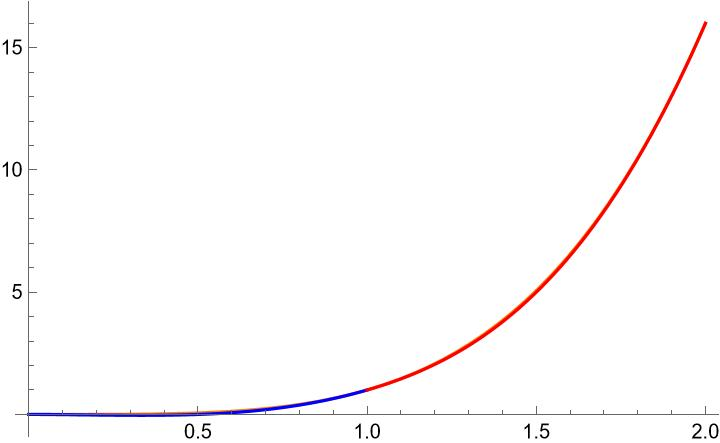
\includegraphics[width=150mm]{splinething.jpg}
    \caption{Graph of figures 3.2 and 3.4 with $p_1(x)$ (blue), and $p_2(x)$ (red).}
    \label{fig:spline_example}
\end{figure}
\\\\
\begin{figure}[htp]
    \centering
    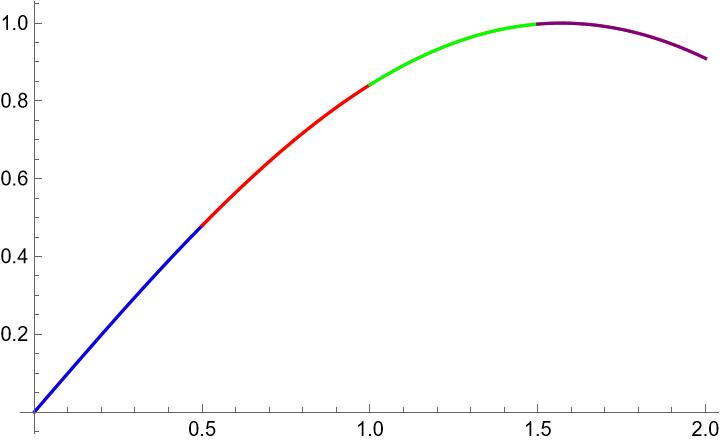
\includegraphics[width=150mm]{splinething2.jpg}
    \caption{Graph of figures 3.5 with $p_1(x)$ (blue), and $p_2(x)$ (red), $p_3(x)$ (green), and $p_4(x)$ (purple).}
    \label{fig:spline_example}
\end{figure}
\\\\
\begin{figure}[htp]
    \centering
    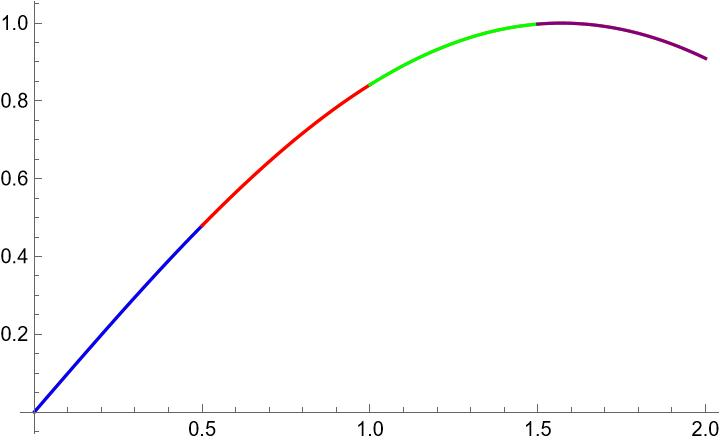
\includegraphics[width=150mm]{splinething3.jpg}
    \caption{Graph of figures 3.6 with $p_1(x)$ (blue), $p_2(x)$ (red), $p_3(x)$ (green) and $p_4(x)$ (purple).}
    \label{fig:spline_example}
\end{figure}
\chapter{Data Collection and Processing}
\label{chapter4}
\thispagestyle{empty}
%\lstset{basicstyle={\ttfamily,\small}, frame=lines}
%I. Introduce methodology
%II. Data
%(a). Table of functions $\{0,1,2\}$
%(b). Table of functions $\{13 data points\}$

%[For each part, describe the Nintegrate and Nmaximize functions and how each of the bounds was calculated.]
\section{Calculation of Splines}
To calculate the cubic splines, we generalized the conditions given in theorem 3.2 and formulated them into Mathematica as code using for loops to iterate the interpolation conditions to minimize redundant code for the splines in $S(K, P_{n})$. We also did the same formulation of the interpolation conditions in order to write the code to construct the splines in $S(MP, P_{n})$. The full codes for each algorithm are provided in appendices A and B.\\\\
In the examples of cubic spine interpolation provided in section 3, we omitted the fact that for small partitions such as $\{0,1,2\}$ one can solve for the coefficients $a_{o},...,d_{1}$ by using Gaussian elimination to solve the system of $8$ linear equations. However, for larger partitions, this can be tedious, hence in the codes we utilized Mathematica's built-in \emph{Solve} function. To solve systems of linear equations, we concatenated each of the vectors into a single matrix for the first argument of the function, and the column vector containing the coefficient variables was used in the second argument. This in turn allowed us to distinguish if the splines generated by each algorithm for the same partition had the same coefficients or not.
\section{Calculation of the $L^2$ and $L^{\infty}$ Error Values}
In this section, we provide a detailed explanation of the data collection process that was used for the Kreyszig and Mhaskar-Pai cubic spline interpolation methods. The Mathematica language served as the basis for all the programs written, including the construction of the cubic splines and the error calculations in the $L^2$ and $L^{\infty}$ norms.
\\\\
For each of the $L^2$ values using definition 2.1, we integrated the difference squared between the function and its spline on the appropriate sub-interval and took the square root of the sum of these integrals using the \emph{Nintegrate} built-in functions. We can take the summation of the square root of each integral since the property of definite integrals allows us to do so. This is symbolically represented by the following equation: \\\\
\centerline{$\displaystyle{\left(\int_{a}^{b} |f(x)-p(x)|^2 \mathrm{d}x\right)^\frac{1}{2} = \left(\int_{x_{0}}^{x_{1}} |f(x)-p_{0}(x)|^2 \mathrm{d}x \right)^\frac{1}{2} + ... + \left(\int_{x_{n-1}}^{x_{n}} |f(x)-p_{n-1}(x)|^2 \mathrm{d}x\right)^\frac{1}{2}}$}.\\\\
To calculate the $L^{\infty}$ values, we know that we must take the maximum value of the sup-norm out of the sub-intervals within $[0,2]$ according to definition 2.2. Hence we took the differences between the original function and the respective cubic spline piece and took the maximum with the \emph{Nmaximize} function in Mathematica to identify which sub-interval provided the maximum value. That is, we calculated \\\\
\centerline{$\displaystyle{\max_{x \in [x_{i}, x_{i+1}]}|f(x)-p_{i}(x)|}$}\\\\
 for $i = 0,1,...,n-1$ and then took the maximum over all $i$. The $L^2$ and $L^{\infty}$ error bounds were calculated using the formulas provided from theorems 3.3 and 3.4 respectively for each of the $L^2$ and $L^{\infty}$ norms. The \emph{Nmaximize} function and its counterpart \emph{Nminimize} use global optimization algorithms such as Nelder-Mead, random search, simulated annealing, and differential evolution in order to approximate the maxima and minima over a given domain \cite{key10}. Meanwhile, the \emph{Nintegrate} function uses special algorithms called \emph{integration strategies} which include singularity handling, oscillatory strategies, and crude Monte Carlo strategies \cite{key11}. More information about these functions and their algorithms can be found in the official Wolfram language documentation.

\section{Calculation of the $L^2$ and $L^{\infty}$ Relative Errors}
In numerical analysis, it is common practice to compute the relative error between approximations and actual values \cite[pg. 17]{key3}. The relative errors for each of the cubic spline interpolation methods were calculated in the same environment as the $L^2$ and $L^{\infty}$ error values. We define the $L^2$ relative error as\\\\
\centerline{$\displaystyle{\frac{\|f(x)-p(x)\|_{2}}{\|f(x)\|_{2}}}$}\\\\
We also define the $L^{\infty}$ relative error in a similar fashion\\\\
\centerline{$\displaystyle{\frac{\|f(x)-p(x)\|_{\infty}}{\|f(x)\|_{\infty}}}$}\\\\
To compute these particular values, we first initialized a variable in the code that would use the \emph{Nintegrate} function to calculate the $L^2$ integral of the original function we are approximating. After retrieving both the error values and norm calculations of each function, we imported the data into an Excel spreadsheet as an auxiliary tool to compute serialized divisions required to obtain the relative error in $L^2$ and $L^{\infty}$. Suppose that we wanted to find the $L^2$ relative error of $S(K, P_{n})$ where the cell E7 holds the $L^2$ norm calculation and F7 contains the $L^2$ value. Then our formula in Excel is written as\\\\
=F7/E7\\\\
To organize the data, we performed a sort of each column in the spreadsheet to order each of the functions' approximations by their relative errors. For example, we first sorted the data by the $L^2$ relative error column to visually inspect which splines performed well in their approximations versus the splines that performed poorly within the partition. Then we repeated the sort with the $L^{\infty}$ column to confirm our results from the $L^{\infty}$ sort. This in turn allowed us to make certain observations and conjectures about the data regarding the accuracy of the cubic spline approximations in each of the norms.


% Chapter 4 File

\chapter{Analysis}
\label{chapter5}
\thispagestyle{empty}

In this section, we provide an analytical dissection of the data we obtained after calculating each test function's respective cubic spline, norm, and error. We used the Excel spreadsheet's sorting and statistical functionalities, the data had arisen to some interesting observations that we believe may support our assertions regarding how well each type of cubic spline approximated the functions. For the curious reader, we have included tables of the cubic spline estimates and their relative error values in Appendices C, D, and E.

\section{Special Observations and Algorithm Analysis}
One of the key observations made from the collected data about both cubic spline interpolation algorithms for $S(K, P_{n})$ and $S(MP, P_{n})$ is that they can sometimes produce identical cubic spline approximations under the same partition even though both algorithms have different interpolation conditions. For example, recall equations 3.2 and 3.4 from chapter 3. It is obvious that the Kreyszig algorithm includes the boundary condition that the first and second derivatives of each piece of the spline must interpolate with each other at each of the intermediate points, expressed symbolically as\\\\
$p_{1}'(1) = p_{2}'(1)$ \text{and}
$p_{1}''(1) = p_{2}''(1)$\\\\
which is directly given by the $S(K, P_{n})$ example. On the other hand, the Mhaskar-Pai algorithm uses only the first derivative in its interpolation conditions and avoids matching the first derivatives of each of the spline pieces with each other as done in Kreyszig's algorithm. In appendix F, we provide a table of cases in which both algorithms produce the same spline. From the data, we note that the function $x^4$ had the same cubic spline on the partition $\{0,0.5,1,1.5,2\}$.

\section{Balanced Partition Analysis}
Our first group of observations from the data is in regard to the best and worst function approximation errors. The first observation that the data supports is that for the balanced partition $\{0, 0.5, 1, 1.5, 2\}$, the functions $\cos(x)$, $\ln(x+1)$, and $x^4$ had the least error in both the Kreyszig and Mhaskar-Pai cubic splines. Since these approximations both had the least relative $L^2$ and $L^{\infty}$ errors, it is clear that the splines approximated their original functions very well in these norms. 
\\\\
On the other hand, we observe that there are approximations that did not perform so well on the same balanced partition $\{0, 0.5, 1, 1.5, 2\}$ for the Kreyszig splines. For example, the sorting procedure we conducted verified that the functions $x^2\cos(x)$, $\sin(x)$, and $x^4\cos(x)$ were approximated poorly since they have the greatest $L^2$ and $L^{\infty}$ relative errors out of the other functions tested. We currently do not have a valid mathematical explanation for this phenomenon as more research is needed in order to arrive at a mathematically appropriate conclusion. The Mhaskar-Pai splines did not approximate the functions $x^3\sin(x)$, $x^2\cos(x)$, and $x^4\cos(x)$ well either. It is interesting to note here that the data supports the conjecture that these higher-power polynomial-trigonometric functions have poor approximations in these norms.

\section{Unbalanced Partition Analysis}
We now shift our focus to the unbalanced partition $\{0, 0.001, 0.01, 0.1, 2\}$. We are particularly interested in testing our cubic spline approximations using this partition choice since it does not divide the interval into equidistant sub-intervals. Once again after sorting the data, we came to the conclusion that the functions $x^4$, $\ln(x+1)$, and $\cos(x)$ were approximated very well in both the Kreyszig and Mhaskar-Pai spline algorithms. The relative $L^2$ and $L^{\infty}$ errors were about $1 \times 10^{1}$ greater than their balanced partition relative errors.
\\\\
In the Kreyszig spline test cases, the worst performing approximations were given from the functions $x^3\sin(x)$, $x^3\cos(x)$, and $x^4\cos(x)$. The only notable difference was the larger relative errors of the approximations and the absence of $\sin(x)$. However, we also noticed that there was a decrease in approximation accuracy with the Mhaskar-Pai splines in the unbalanced partition. For example, the functions that did not have particularly good approximations were $x^4\sin(x)$, $x^4\cos(x)$, and $x^3\cos(x)$, which are once again higher-power polynomial-trigonometric functions that have greater relative errors in the $L^2$ and $L^{\infty}$ norms. 

\section{Sharpness of Error Bounds}
We now introduce the other measure of approximation accuracy, the $L^2$ and $L^{\infty}$ error bounds that come from using theorems 3.4 and 3.5. An error bound is considered to be \emph{sharp} if the bound $b$ is impossible to improve.
For example, in theorem 3.5 Mhaskar-Pai says that the error in the spline approximation of the function $\sin(x)$ on the partition $\{0,0.5,1,1.5,2\}$ is at worst 0.01953125. The actual error is 0.000167649. Since $0.01953125-0.000167649 = 0.019363601$ is the smallest difference between one of our functions' $L^{\infty}$ error on $\{0,0.5,1,1.5,2\}$ and the maximum error from theorem 3.5, we say that $\sin(x)$ has the sharpest $L^{\infty}$ error bound on $\{0,0.5,1,1.5,2\}$. Using this definition of sharpness, we noticed that $\sin(x)$, $\cos(x)$, and $\ln(x+1)$ had the sharpest $L^2$ and $L^{\infty}$ error bounds on the partition $\{0,0.5,1,1.5,2\}$. We have provided the data for these $L^2$ and $L^{\infty}$ error bounds in appendices C and D.

% Conclusion File

\chapter{Concluding Remarks and Future Work}
\thispagestyle{empty}
\section{Summary}

In this thesis, we introduced the classical theory of cubic spline interpolation and focused on two types of cubic spline interpolation from Kreyszig and from Mhaskar-Pai. After constructing the cubic splines for each model using Mathematica code, data analysis was performed based on the two different measures of relative error, as well as Mhaskar-Pai error-bound calculations. For both the Kreyszig and Mhaskar-Pai splines we concluded that the cubic spline approximations for both models of the functions $x^4$, $\ln(x+1)$, and $\cos(x)$ performed the best with the minimum amount of $L^2$ and $L^{\infty}$ relative error. The functions $x^4$, $\ln(x+1)$, and $\cos(x)$ were closest to the maximum error predicted by Mhaskar-Pai.
\section{Future Work}
We conclude this paper by providing some insight into how we can approach more immediate future work and present some prospective ideas for distant future work. Due to the limited time we had, it would be beneficial to continue running more mixtures of elementary functions with the same partitions and intervals that we presented in the data tables. For example, we would like to further test the conjecture that $x^n\sin(x)$ has a worse-performing spline approximation than $x^n$ for larger values of $n$. In addition, we can also consider testing the functions we had with a greater amount of unbalanced partitions, and also include different intervals such as $[-4,4]$. These are merely a few possibilities that can be studied in order to develop more conjectures about the algorithms used in cubic spline interpolation.\\\\
It is believed that this research will provide the theoretical groundwork for deeper research to be implemented on the type of function class we investigated. As mentioned previously, cubic spline interpolation is a useful technique that allows scientists to make predictions about data sets. Future work could also consider the same analysis that we conducted in this thesis to cubic splines of multivariable functions in normed spaces. Our hope is that the next curious mind who stumbles upon this paper within the university community will be enlightened in the way mathematics research is conducted and can have a starting place in learning about the power of mathematics and its numerous real-world applications.


% $$$$$$$$$$$$$$$$$  Reference style  Starts $$$$$$$$$$$$$$

\begin{onehalfspacing}
	\renewcommand*\bibname{\centerline{REFERENCES}} 
    \phantomsection
	\addcontentsline{toc}{chapter}{References}
	\newcommand{\BIBdecl}{\setlength{\itemsep}{0pt}}%To control space between bibliography entries
		\bibliographystyle{plain}
		\bibliography{References}
\end{onehalfspacing}

% $$$$$$$$$$$$$$$$$  Reference style Ends  $$$$$$$$$$$$$$


% $$$$$$$$$$$$$$$$$  include Appendices   $$$$$$$$$$$$$$

\appendix
		\newpage
		\begingroup
			\let\cleardoublepage\clearpage
			\begin{center}
			\vspace*{2\baselineskip}
			{ \textbf{{\large APPENDICES}}} 
            % Fixes the numbering of "new" section created with "\addcontentsline."
            % You need to add the "\phantomsection" before *every* "\addcontentsline."
            %\clearpage
            \phantomsection
			\addcontentsline{toc}{chapter}{Appendices} 
			\end{center}
            %\clearpage
            
% Appendix A File

\refstepcounter{chapter}%
\chapter*{\thechapter \quad Generalized Cubic Spline Interpolation Code (Kreyszig)}
\label{appendixA}

\section{Mathematica Code for $S(K, P_{n})$}
\begin{lstlisting}
xval = {0, 0.5, 2}         
F[s_]:= Sin[s]        
yval = F[xval]
yvalprime = F'[xval]
yvaldoubprime = F''[xval]      

numparts = Length[xval]
n = numparts-1                 

Do[{xx[k-1]=xval[[k]],               
yy[k-1]=yval[[k]],
yyprime[k-1]=yvalprime[[k]],
yydoubprime[k-1]=yvaldoubprime[[k]]},
{k,1,numparts}]

Table[{xx[k],yy[k]},{k, 0, n}];
Unknowns=Table[{a[k],b[k],c[k],d[k]},{k,0,n-1}] // Flatten           

Do[P[k][x_]= a[k]*(x)^3+b[k]*(x)^2+c[k]*(x)+d[k], {k,0,n-1}]

Do[EquationA[k] = P[k][xx[k]] == yy[k] , {k,0,n-1}]
TableA=Table[EquationA[k],{k,0,n-1}]

Do[EquationB[k] =  P[k][xx[k+1]] == yy[k+1] , {k, 0, n-1}]  
TableB=Table[EquationB[k],{k,0,n-1}]

EquationC = { P[0]'[xx[0]]== yyprime[0]}
EquationD = {P[n-1]'[xx[n]]== yyprime[n]}

Do[EquationE[k] =  P[k-1]'[xx[k]] == P[k]'[xx[k]] , {k,1,n-1}]
TableE=Table[EquationE[k],{k,1,n-1}]

Do[EquationF[k] =  P[k-1]''[xx[k]] == P[k]''[xx[k]] , {k,1,n-1}]
TableF=Table[EquationF[k],{k,1,n-1}]

AllEquationsToSolve=Join[TableA,TableB,EquationC,EquationD,TableE,TableF]

Solve[AllEquationsToSolve, Unknowns] 
\end{lstlisting}

Note that the function definition and partition points are the only lines of the code that are updated for each iteration. For example, one can run this code to find the coefficients of the cubic spline that approximates $f(x)=x^4$ on $[0,2]$ with the following partition points $\{0,1,2\}$.
            
% Appendix B File

\refstepcounter{chapter}%
\chapter*{\thechapter \quad Generalized Cubic Spline Interpolation Code (Mhaskar and Pai)}
\label{appendixB}

\section{Mathematica Code for $S(MP, P_{n})$}
\begin{lstlisting}
xval = {0, 0.001, 0.01, 0.1, 2}         
F[s_]:= s^4*Cos[s]
yval = F[xval]
yvalprime = F'[xval]
yvaldoubprime = F''[xval]      

numparts = Length[xval]  
n = numparts-1                 

Do[{xx[k-1]=xval[[k]],               
yy[k-1]=yval[[k]],
yyprime[k-1]=yvalprime[[k]],
yydoubprime[k-1]=yvaldoubprime[[k]]},
{k,1,numparts}]

Table[{xx[k],yy[k]},{k, 0, n}];
Unknowns=Table[{a[k],b[k],c[k],d[k]},{k,0,n-1}] // Flatten           

Do[P[k][x_]= a[k]*(x)^3+b[k]*(x)^2+c[k]*(x)+d[k], {k,0,n-1}]             

Do[EquationA[k] = P[k][xx[k]] == yy[k] , {k,0,n-1}]
TableA=Table[EquationA[k],{k,0,n-1}]

Do[EquationB[k] =  P[k][xx[k+1]] == yy[k+1] , {k, 0, n-1}]  
TableB=Table[EquationB[k],{k,0,n-1}] 

Do[EquationC[k] = P[k]'[xx[k]] == yyprime[k] , {k,0,n-1}]
TableC=Table[EquationC[k],{k,0,n-1}]

Do[EquationD[k] =  P[k]'[xx[k+1]] == yyprime[k+1] , {k, 0, n-1}]  
TableD=Table[EquationD[k],{k,0,n-1}] 

AllEquationsToSolve=Join[TableA,TableB,TableC,TableD]

Solve[AllEquationsToSolve, Unknowns] 
\end{lstlisting}

            
% Appendix C File

\refstepcounter{chapter}%
\chapter*{\thechapter \quad Table of $L^2$ and $L^{\infty}$ Error Bounds I}
\label{appendixC}

\section{Partition $\{0,1,2\}$}
\begin{tabular}{lllll}
Function    & $L^2$ Bound & $L^{\infty}$ Bound & $L^2$ Error      & $L^{\infty}$ Error \\
%
$x^4$       & 30.35786554 & 0.3125             & 0.056343589 & 0.0625       \\
$sin(x)$    & 1.09050447  & 0.013020833        & 0.002061407 & 0.00310302   \\
$cos(x)$    & 0.90044378  & 0.013020833        & 0.399684    & 0.681973     \\
$x^2sin(x)$ & 3.460722468 & 0.177522135        & 0.022391137 & 0.0278455    \\
$x^2cos(x)$ & 5.867145814 & 0.232785156        & 0.043717205 & 0.0497168    \\
$x^3sin(x)$ & 7.327966976 & 0.709542969        & 0.140189051 & 0.19088      \\
$x^3cos(x)$ & 14.63512897 & 0.63094401         & 0.063144731 & 0.091101     \\
$e^{-x^2}$  & 1.367402647 & 0.15625            & 1.478713209 & 2.38103      \\
$ln(x+1)$   & 0.566558029 & 0.078125           & 0.00323539  & 0.00478147  
\end{tabular}


            
% Appendix D File

\refstepcounter{chapter}%
\chapter*{\thechapter \quad Table of $L^2$ and $L^{\infty}$ Error Bounds II}
\label{appendixD}

\section{Partition $\{0, 0.5,1,1.5,2\}$}
\begin{tabular}{lllll}
Function    & $L^2$ Bound & $L^{\infty}$ Bound & $L^2$ Error          & $L^{\infty}$ Error\\
%
$x^4$       & 30.35786554 & 0.46875            & 0.003521477     & 0.00390625   \\
$sin(x)$    & 1.09050447  & 0.01953125         & 0.010833343     & 0.000167649  \\
$cos(x)$    & 0.90044378  & 0.01953125         & 0.0001031607387 & 0.000168202  \\
$x^2sin(x)$ & 3.460722468 & 0.266283203        & 0.001850955     & 0.00279474   \\
$x^2cos(x)$ & 5.867145814 & 0.349177734        & 0.033876803     & 0.124988     \\
$x^3sin(x)$ & 7.327966976 & 1.064314453        & 0.005961173     & 0.00947933   \\
$x^3cos(x)$ & 14.63512897 & 0.946416016        & 0.005031929     & 0.00669749   \\
$e^{-x^2}$  & 1.367402647 & 0.234375           & 0.001561177     & 0.00233593   \\
$ln(x+1)$   & 0.566558029 & 0.1171875          & 0.0002572419925 & 0.000546376 
\end{tabular}
            
% Appendix E File

\refstepcounter{chapter}%
\chapter*{\thechapter \quad Table of $L^2$ and $L^{\infty}$ Error Bounds III}
\label{appendixE}

\section{Partition $\{0,0.001,0.01,0.1,2\}$}
\begin{tabular}{lllll}
Function    & $L^2$ Bound & $L^{\infty}$ Bound & $L^2$ Error          & $L^{\infty}$ Error\\
%
$x^4$       & 5.603216082 & 1.005056877            & 0.757722     & 0.852309   \\
$sin(x)$    & 0.180027389  & 0.04187737         & 0.0253919     & 0.0288343  \\
$cos(x)$    & 0.148650965  & 0.04187737         & 0.0149826 & 0.0171375  \\
$x^2sin(x)$ & 2.280493123 & 0.570943498        & 0.367591     & 0.418711   \\
$x^2cos(x)$ & 2.393700652 & 0.748679431        & 0.0685228     & 0.088225     \\
$x^3sin(x)$ & 8.122818181 & 2.282019329        & 0.756019     & 0.872238   \\
$x^3cos(x)$ & 5.549725343 & 2.029230773        & 0.626801     & 0.724703   \\
$e^{-x^2}$  & 1263.298857 & 1051.754332           & 25.9381     & 29.2647   \\
$ln(x+1)$   & 0.374295181 &  0.251264219         & 0.0154627 & 0.0174493 
\end{tabular}
            % Appendix F File

\refstepcounter{chapter}%
\chapter*{\thechapter \quad Table of Functions and Their Relative Errors}
\label{appendixF}

\section{Kreyszig Spline Interpolation for \newline
Partition $\{0,0.5,1,1.5,2\}$}
\tiny{\begin{tabular}{lllllllll}
Function                                     &  $L^{\infty}$ Norm & $L^2$ Norm  & $L^2$           & $L^{\infty}$       & $L^2$ Relative Error & $L^{\infty}$ Relative Error \\
$x^4$                     & 16                      & 7.54257                & 0.003521477                     & 0.00390625                      & 0.000466886                         & 0.000244141                           \\
$sin(x)$                                      & 1                       & 1.0905                & 0.010833343                     & 0.000167649                     & 0.00993429                          & 0.000167649                           \\
$cos(x)$                                      & 1                       & 0.900444              & 0.0001031607387 & 0.000168202 & 0.000114567                         & 0.000168202                           \\
$x^2sin(x)$               & 3.63719                 & 2.42378               & 0.001850955                     & 0.00279474                      & 0.000763665                         & 0.000768379                           \\
$x^2cos(x)$               & 1.66459                 & 0.724767              & 0.038876803                     & 0.124988                        & 0.046741647                         & 0.075086358                           \\
$x^3sin(x)$               & 7.27438                 & 4.10838               & 0.005961173                     & 0.00947933                      & 0.001450979                         & 0.001303112                           \\
$x^3cos(x)$               & 3.32917                 & 1.18613               & 0.005031929                     & 0.00669749                      & 0.004242308                         & 0.00201176                            \\
$e^{-x^2}$ & 1                       & 0.791592              & 0.001561177                     & 0.00233593                      & 0.001972199                         & 0.00233593                            \\
$ln(x+1)$                                      & 1.09861                 & 1.01448               & 0.0002572419925 & 0.000546376 & 0.00025357                          & 0.000497334                           \\
$x^4sin(x)$               & 14.5488                 & 7.22793               & 0.01981 & 0.0405855 & 0.002740757                         & 0.002789612                           \\
$x^4cos(x)$               & 6.65835                 & 2.15544               & 0.0136382 & 0.0269258 & 0.006327339                         & 0.004043915                          

\end{tabular}}

\section{Kreyszig Spline Interpolation for \newline
Partition $\{0,0.001,0.01,0.1,2\}$}
\tiny{\begin{tabular}{llllllll}
Function        & $L^{\infty}$ Norm & $L^{2}$ Norm & $L^{2}$        & $L^{\infty}$   & $L^{2}$ Relative Error & $L^{\infty}$ Relative Error \\
$x^{4}$       & 16                            & 7.54257                  & 0.753015 & 0.852309 & 0.099836658         & 0.053269313              \\
$sin(x)$      & 1                             & 1.0905                   & 0.0253792 & 0.0288343 & 0.023272994         & 0.0288343              \\
$cos(x)$      & 1                             & 0.900444                 & 0.0149723 & 0.0171375 & 0.016627686         & 0.0171375              \\
$x^{2}sin(x)$ & 3.63719                       & 2.42378                  & 0.367392 & 0.418711 & 0.151578114         & 0.115119364              \\
$x^{2}cos(x)$ & 1.66459                       & 0.724767                 & 0.0684972 & 0.0882225 & 0.09450927        & 0.052999537              \\
$x^{3}sin(x)$ & 7.27438                       & 4.10838                  & 0.755778 & 0.872238 & 0.183960101         & 0.119905476             \\
$x^{3}cos(x)$ & 3.32917                       & 1.18613                  & 0.626398 & 0.724703 & 0.528102316         & 0.217682786              \\
$e^{-x^2}$    & 1                             & 0.791592                 & 0.125958 & 0.146861 & 0.15911985         & 0.146861              \\
$ln(x+1)$     & 1.09861                       & 1.01448                  & 0.0154493 & 0.0174493 & 0.015228787         & 0.01588307              \\
$x^{4}sin(x)$ & 14.5488                       & 7.22793                  & 0.869449 & 1.06411        & 0.12029018        & 0.07314074              \\
$x^{4}cos(x)$ & 6.65835                       & 2.15544                  & 2.42863        & 2.7848         & 1.126744423          & 0.418241757             
\end{tabular}}

\section{Mhaskar-Pai Interpolation for
\newline
Partition $\{0,0.5,1,1.5,2\}$}
\tiny{\begin{tabular}{llllllll}
Function      & $L^{\infty}$ Norm & $L^{2}$ Norm & $L^{2}$        & $L^{\infty}$   & $L^{2}$ Relative Error & $L^{\infty}$ Relative Error \\

%
$x^{4}$       & 16                            & 7.54257                  & 0.003521477    & 0.00390625     & 0.000466886            & 0.000244141                 \\
$sin(x)$      & 1                             & 1.0905                   & 0.010715379    & 0.0401195      & 0.009826116            & 0.0401195                   \\
$cos(x)$      & 1                             & 0.900444                 & 0.00009271080304 & 0.000157036 & 0.000102961            & 0.000157036                 \\
$x^{2}sin(x)$ & 3.63719                       & 2.42378                  & 0.001422177    & 0.00209826     & 0.00058676             & 0.00057689                  \\
$x^{2}cos(x)$ & 1.66459                       & 0.724767                 & 0.128334318    & 0.182018       & 0.177069759            & 0.109347046                 \\
$x^{3}sin(x)$ & 7.27438                       & 4.10838                  & 0.047919437    & 0.10125        & 0.011663828            & 0.013918712                 \\
$x^{3}cos(x)$ & 3.32917                       & 1.18613                  & 0.003276185    & 0.00499725     & 0.002762079            & 0.00150105                  \\
$e^{-x^2}$    & 1                             & 0.791592                 & 0.0008056204565 & 0.00134145     & 0.001017722            & 0.00134145                  \\
$ln(x+1)$     & 1.09861                       & 1.01448                  & 0.000198022878 & 0.000423712 & 0.000195196            & 0.00038568                  \\
$x^{4}sin(x)$ & 14.5488                       & 7.22793                  & 0.0154138 & 0.03222238 & 0.002132533            & 0.002214877                 \\
$x^{4}cos(x)$ & 6.65835                       & 2.15544                  & 2.21213        & 4.00015        & 1.026300894            & 0.600771963                
\end{tabular}}

\section{Mhaskar-Pai Interpolation for
\newline
Partition $\{0,0.001,0.01,0.1,2\}$}
\tiny{\begin{tabular}{llllllll}
Function   & $L^{\infty}$ Norm & $L^{2}$ Norm & $L^{2}$        & $L^{\infty}$   & $L^{2}$ Relative Error & $L^{\infty}$ Relative Error \\
%
$x^{4}$       &  16                            & 7.54257                  & 0.715683 & 0.814506 & 0.094887086         & 0.050906625              \\
$sin(x)$      &  1                             & 1.0905                   & 0.0242887 & 0.0277475 & 0.022272994         & 0.0277475              \\
$cos(x)$      &  1                             & 0.900444                 & 0.0139979 & 0.0161115 & 0.015545553         & 0.0161115              \\
$x^{2}sin(x)$ &  3.63719                       & 2.42378                  & 0.350294 & 0.401374 & 0.144523843         & 0.110352772              \\
$x^{2}cos(x)$ &  1.66459                       & 0.724767                 & 0.0700292 & 0.0897031 & 0.096623053         & 0.053889006             \\
$x^{3}sin(x)$ &  7.27438                       & 4.10838                  & 0.736298 & 0.853713 & 0.179218573         & 0.117358868              \\
$x^{3}cos(x)$ &  3.32917                       & 1.18613                  & 0.590717 & 0.687323 & 0.498020453         & 0.206454762             \\
$e^{-x^2}$    &  1                             & 0.791592                 & 0.121717 & 0.142521 & 0.153762292         & 0.142521              \\
$ln(x+1)$     & 1.09861                       & 1.01448                  & 0.0142342 & 0.0161619 & 0.014031031         & 0.014711226              \\
$x^{4}sin(x)$ & 14.5488                       & 7.22793                  & 1.98575  & 4.94078  & 0.274732876         & 0.339600517              \\
$x^{4}cos(x)$ & 6.65835                       & 2.15544                  & 0.67361 & 1.68913  & 0.312516238         & 0.253685973             
\end{tabular}}
            
% Appendix G File

\refstepcounter{chapter}%
\chapter*{\thechapter \quad Table of Identical Splines}
\label{appendixG}

\section{Partition $\{0,0.5,1,1.5,2\}$}
\small{\begin{tabular}{ll}
Function    & $S(K,P_{n})=S(MP,P_{n})$ \\
$x^4$       & yes                      \\
$sin(x)$    & no                       \\
$cos(x)$    & no                       \\
$x^2sin(x)$ & no                       \\
$x^2cos(x)$ & no                       \\
$x^3sin(x)$ & no                       \\
$x^3cos(x)$ & no                       \\
$e^{-x^2}$  & no                       \\
$ln(x+1)$   & no                       \\
$x^4sin(x)$ & no                       \\
$x^4cos(x)$ & no                      
\end{tabular}}

\section{Partition $\{0,0.001,0.01,0.1,2\}$}
\small{\begin{tabular}{ll}
Function    & $S(K,P_{n})=S(MP,P_{n})$ \\
$x^4$       & no                      \\
$sin(x)$    & no                       \\
$cos(x)$    & no                       \\
$x^2sin(x)$ & no                       \\
$x^2cos(x)$ & no                       \\
$x^3sin(x)$ & no                       \\
$x^3cos(x)$ & no                       \\
$e^{-x^2}$  & no                       \\
$ln(x+1)$   & no                       \\
$x^4sin(x)$ & no                       \\
$x^4cos(x)$ & no                      
\end{tabular}}
		\endgroup
% $$$$$$$$$$$$$$$$$  Appendix ends  $$$$$$$$$$$$$$

\end{document}

